\chapter{绪论}

\section{操作系统基本概念}

    \emph{任何计算机系统都包含一个名为操作系统的基本程序集合。}在这个集合中,最重要的程序称为内核(kernel)。启动后,内核中包含了系统运行所必不可少的很多核心过程(procedure),和其他一些不太重要的实用程序。

    \emph{系统根本的样子和能力还是由内核决定,内核也为操作系统中所有事情提供了主要功能,并决定高层软件的很多特性。}

    操作系统必须完成两个主要目标:

\begin{itemize}
    \item [1)] 与硬件部分交互,为包含在硬件平台上的所有底层可编程部件提供服务
    \item [2)] 为运行在计算机系统上的应用程序提供执行环境
\end{itemize}

    \emph{类Unix系统把与计算机物理组织相关的所有底层细节都对用户运行的程序隐藏起来,硬件为CPU引入了至少两种不同的执行模式:非特权模式(用户态(User Mode)和特权模式(Kernel Mode))}。

\section{多用户系统}

    \emph{多用户系统(multiuser system)就是一台能并发和独立地执行分别属于两个或多个用户的若干应用程序的计算机。}

    并发(concurrently)意味着几个应用程序能够同时处于活动状态并竞争各种资源。独立(independently)意味着每个应用程序能够执行自己的任务,而无需考虑其他用户的应用程序在做什么。

    多用户操作系统必须包含:

\begin{itemize}
    \item [1)] 核实用户身份的认证机制
    \item [2)] 防止有错误的用户程序妨碍其他应用程序在系统中运行的保护机制
    \item [3)] 防止有恶意的用户程序干涩或窥视其他用户的活动的保护机制
    \item [4)] 限制分配给每个用户的资源数的记账机制
\end{itemize}

\section{用户和组}

    操作系统必须保证用户空间的私有部分仅仅对于其拥有者是可见的。

    所有的用户由一个唯一的数字来表示,这个数字叫用户标识符(User ID, UID)。

    为了和其他用户有选择地共享资料,每个用户是一个或多个用户组的一名成员,组由唯一的用户组标识符(user group ID)标识。每个文件也恰好与一个组相对应。

    \emph{任何类Unix操作系统都有一个特殊的用户,root(超级用户(superuser))}。系统管理员能够通过root账号登陆,值得一提的是:\emph{root几乎无所不能,其能访问系统中的每一个文件,能干涉每一个正在执行的用户程序}。

\section{进程}

    \emph{所有的操作系统都有一种基本的抽象:进程(process)。一个进程可以定义为:"程序运行时的一个实例",或者一个运行程序的"执行上下文"}。

    传统的操作系统中,\emph{一个进程在地址空间中(address space)执行一个单独的指令序列。}现代操作系统允许具有多个执行流的进程,也就是在相同的地址空间可执行多个指令序列。

    \emph{允许进程并发活动的系统称为多道程序系统(multiprogramming)或多处理系统(multiprocessing)}。值得注意的是:几个进程能够并发地执行同一个程序,而同一个进程能顺序的执行几个程序。

    调度程序(scheduler)的部分决定哪个进程能执行,一些操作系统只允许有非抢占式(nonpreemptable)进程,\emph{也就是说,只有当进程自愿放弃时,调度程序才能被调用。但是,多用户系统中的进程必须是抢占式的(preemptable)}。

\section{内核体系结构}

    大部分Unix内核都是单块结构:\emph{每一个内核层都被集成到整个内核程序中,并代表当前进程在内核态下运行。}

    \emph{微内核(microkernel)操作系统只需要内核有一个很小的函数集(几个同步原语\footnote[1]{原语(primitive)是计算机科学中的一个概念,它指的是一组基本的操作或指令,可以直接在计算机硬件上执行。原语通常是由计算机硬件提供的,用于支持高级编程语言或操作系统的功能},一个简单的调度程序和进程间通信)}。

    Linux内核提供了模块(module)用于达到微内核理论上的很多优点且不影响性能。\emph{模块是一个目标文件,其代码可以在运行时链接到内核或从内核解除链接。这种目标代码通常由一组函数组成,用来实现文件系统、驱动程序或其他内核上层功能。}

    使用模块的主要优点:

\begin{itemize}
    \item [1)] 模块化方法
    \subitem 任何模块都能在运行时被链接或解除链接。这要求程序员提出良定义的软件接口以访问由模块处理的数据结构
    \item [2)] 平台无关性
    \subitem 即使模块依赖于某些特殊的硬件特点,但它不依赖于某个固定的硬件平台
    \item [3)] 节省内存使用
    \subitem 当需要模块时,就链接;不需要时,则解除
    \item [4)] 无性能损失
    \subitem 模块的目标代码一旦被链接进内核,起作用与静态链接的内核的目标代码完全对等。因此无需显式的进行消息传递\footnote[1]{模块被链接或解除时,都有一定的性能下降。但是在微内核中也是如此}
\end{itemize}

\section{Unix文件系统概述}

\subsection{文件}

    \emph{Unix文件是以字节序列组成的信息载体(container),内核不解释文件的内容。}

    从用户的观点来看,文件被组织在一个树结构的命名空间内:

\begin{figure}[!htbp]
    \centering
    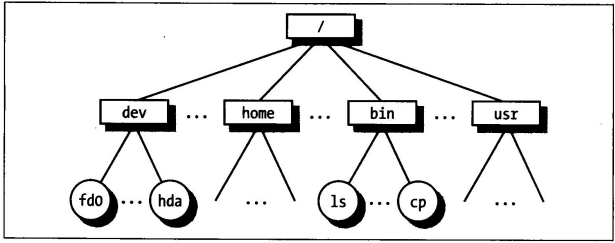
\includegraphics[width=0.6\textwidth]{image/chapter01/目录树结构.png}
    \caption{目录树结构}
\end{figure}

    除叶节点外,所有节点都表示目录名。目录节点包含它下面文件及目录的所有信息。

    \emph{Unix每个进程都有一个当前工作目录,属于进程执行上下文(execution context),标识出进程所用的当前目录。}

    \emph{路径名(pathname)由斜杠及一列指向文件的目录名交替组成。如果第一个字符是斜杠,那么就是所谓的绝对路径;否则就是所谓的相对路径。}

    当标识文件名时,用符号"."和".."分别标识当前工作目录和父目录。

\subsection{硬链接和软连接}

    \emph{包含在目录中的文件名就是一个文件的硬链接(hard link),或简称连接(link)。}

    使用Unix命令:

\begin{lstlisting}[language=C++]
$ ln P1 P2
\end{lstlisting}

    用来创建一个新的硬链接,即为由路径P1标识的文件创建一个路径名为P2的硬链接。

    硬链接有两方面的限制:

\begin{itemize}
    \item [1)] 不允许给目录创建硬链接,这可能使得目录树编程环形图从而无法通过名字定位一个文件
    \item [2)] 只有在同一文件系统中的文件之间才能创建链接。
\end{itemize}

    为了克服限制,引入\emph{软链接(soft link)[也称符号链接(symbolic link)],符号链接是短文件,这些文件包含另一个文件的任意一个路径名。}

    值得注意的是:\emph{路径名可以指向位于任意一个文件系统的任意文件或目录(哪怕它不存在)}。

    Unix命令:

\begin{lstlisting}[language=C++]
$ ln -s P1 P2
\end{lstlisting}

    创建一个路径名为P2的新软连接,P2指向路径名P1。当执行命令时,文件系统抽取P2的目录部分,并在此创建P2的符号链接属性的新项。因此,任何对P2的引用都可以自动被转换为指向P1的引用。

\subsection{文件类型}

    Unix命令文件可以是以下类型:

\begin{itemize}
    \item 普通文件(regular file)
    \item 目录
    \item 符号链接
    \item 面向块的设备文件(block-oriented device file)
    \item 面向字符的设备文件(character-oriented device file)
    \item 管道(pipe)和命名管道(named pipe)(也叫FIFO)
    \item 套接字(socket)
\end{itemize}

\subsection{文件描述符与索引节点}

    \emph{除了设备文件和特殊文件系统外,每个文件都由字符序列组成。文件内容不包括任何控制信息,如文件长度或文件结束符(end-of-file, EOF)}。

    \emph{文件系统处理文件需要的所有信息都包含在一个名为索引节点(inode)的数据结构中,文件系统用索引节点来标识文件。}

    索引节点(inode)至少包括:

\begin{itemize}
    \item 文件类型
    \item 与文件相关的硬链接个数
    \item 以字节为单位的文件长度
    \item 设备标识符(即包含文件的设备的标识符)
    \item 文件系统中标识的索引节点号
    \item 文件拥有者的UID
    \item 文件的用户组ID
    \item 几个时间戳(改变时间、最后访问时间、最后修改时间)
    \item 访问权限和文件模式
\end{itemize}

\subsection{访问权限和文件模式}

    文件的潜在用户分为三种类型:

\begin{itemize}
    \item 文件所有者
    \item 同组用户(不含所有者)
    \item 其他用户
\end{itemize}

    同时,拥有三种类型的访问权限————读、写以及执行。因此就有九种组合不同的二进制来标记,还有三种额外的标记

\begin{itemize}
    \item suid
    \subitem 进程执行一个文件时通常保持进程拥有者的UID,若设置suid,进程就可以获取该文件拥有者的UID
    \item sgid 
    \subitem 进程执行一个文件时保持进程组的用户组ID,若设置sgid,进程就可以获得该文件用户组ID
    \item sticky
    \subitem 设置sticky标志位相当于向内核发出请求,当程序结束后仍保留在内存\footnote[1]{该标记已经过时,已被其他方法取代}
\end{itemize}

\subsection{文件操作的系统调用}

    \emph{当用户访问一个普通文件或目录文件的内容时,实际上访问的是在硬件块设备上的一些数据。}

\subsubsection{打开文件}

\begin{lstlisting}[language=C++]
/**
* @param path 表示被打开文件的路径
* @param flag 指定文件打开的方式,也可以创建一个不存在的文件
* @param mode 指定新创建文件的访问权限
*/

fd = open(path, flag, mode)
\end{lstlisting}

    该系统调用返回文件描述符(file descriptor)的标识符。一个打开文件对象包括:

\begin{itemize}
    \item 文件操作的一些数据结构;表示文件当前位置的offset字段等等
    \item 进程可以调用的一些内核函数指针,由参数flag决定
\end{itemize}

\subsubsection{访问打开的文件}

    \emph{对于Unix普通文件,可以顺序或随机访问;但设备文件和命名管道文件一般只能顺序访问。}

    内核把文件指针存放在打开文件对象中,也就是,当前位置就是下一次进行读或写的位置。为了修改文件指针的值,必须显式调用lseek()系统调用。

\begin{lstlisting}[language=C++]
/**
* @param fd 表示打开文件的文件描述符
* @param offset 指定一个有符号整数,用于计算文件指针的新位置
* @param whence 指定文件指针新位置的计算方式:offset加0,表示从文件头移动;offset加文件指针当前位置,表示从当前移动等
*/
newoffset = lseek(fd, offset, whence);

/**
* @param fd 表示打开文件的文件描述符
* @param buf 指定在进程地址空间中缓冲区的地址,所读的数据放在该缓冲区
* @param count 表示所读的字节数
*/
nread = read(fd, buf, count);
\end{lstlisting}

    返回值nread的值就是实际所读的字节数。

\subsubsection{关闭文件}

    当进程无需访问文件时,则可以关闭文件资源

\begin{lstlisting}[language=C++]
res = close(fd)
\end{lstlisting}

\subsubsection{更名与删除文件}

    \emph{重新命名和删除并不需要进程打开文件}

\begin{lstlisting}[language=C++]
res = rename(oldpath, newpath);
\end{lstlisting}

    改变文件链接的名字:

\begin{lstlisting}[language=C++]
res = unlink(pathname)
\end{lstlisting}

    \emph{文件真正的被删除时:链接数为0才会被删除。}

\section{Unix内核概述}

    \emph{Unix内核提供了应用可以运行的执行环境。因此,内核需要实现服务与对应接口。}

\subsection{进程/内核模式}

    \emph{程序在用户态下执行时,不能直接访问内核数据结构或内核的程序。}CPU都为从用户态到内核态的转换提供了特殊的指令。\emph{程序大部分时间都在用户态,只有需要内核提供特殊服务时会切换到内核态}。

    \emph{进程是动态的实体,在系统内通常只有有限的生存期。创建、撤销及同步现有进程的任务都委托给内核中的一组例程。}内核本身不是进程,而是进程的管理者。

    规定:\emph{请求内核服务的进程使用所谓系统调用(system call)的特殊编程机制。每个系统调用都设置了一组识别进程请求的参数,然后执行用户--内核态转换。}

    Unix系统包括几个内核线程(kernel thread):

\begin{itemize}
    \item 以内核态运行在内核地址空间
    \item 不与用户直接交互
    \item 在系统启动时创建,一直活跃到系统关闭
\end{itemize}

    在单系统中,任何时候只有一个进程在运行,要么处于用户态,要么处于内核态。

    Unix中,可以通过以下方式激活内核例程:

\begin{itemize}
    \item 调用系统调用
    \item 进程发出异常(exception)信号
    \item 外围设备发出中断(interrupt)信号通知一个事件的发生。每个中断信号都是由中断处理程序(interrupt handler)处理的
    \item 内核线程被执行
\end{itemize}

\subsection{进程实现}

    为了让内核管理进程,每个进程由一个进程描述符(process descriptor)表示,该描述符包含有关进程当前状态的信息。

    内核暂停一个进程的执行,需要保存其相关信息(将相关寄存器保存在进程描述符中):

\begin{itemize}
    \item 程序计数器(PC)和栈指针(SP)
    \item 通用寄存器
    \item 浮点寄存器
    \item 状态寄存器(处理器状态字,Processor Status Word)
    \item 用于跟踪进程对RAM访问的内存管理寄存器
\end{itemize}

    由于保存PC的原因,进程会从它停止的地方恢复执行。Unix内核可以区分很多等待状态,由进程描述符队列实现。

\subsection{可重入内核}

    所有的Unix内核都是可重入的\footnote[1]{\emph{具体来说,可重入函数是指在多个线程同时调用时,不会出现竞争条件或数据不一致的情况。这意味着函数的执行不依赖于外部状态,并且可以在任何时间点被中断和恢复,而不会影响函数的正确性。}}(reentrant),这意味着若干进程可以同时在内核态下执行。

    \emph{提供可重入的一种方式是编写函数,以便这些函数只能修改局部变量,而不能修改全局数据结构,这样的函数叫做可重入函数。}可重入内核可以包含非重入函数,并且利用锁机制保证一次只有一个进程执行一个非重入函数。

    如果一个硬件中断发生,可重入内核能挂起当前正在执行的进程,即使这个进程处于内核态。

    内核控制路径\footnote[2]{\emph{指操作系统内核在执行期间所经过的代码路径。它代表了操作系统的执行流程,包括中断处理、系统调用、任务切换等。内核控制路径通常是由硬件中断或软件触发的事件引发的。当一个事件发生时,例如外部设备的中断请求或用户程序的系统调用,操作系统内核会通过相应的中断处理程序或系统调用处理程序来响应和处理这个事件。}}(kernel control path)表示内核处理系统调用、异常或中断执行的指令序列。

    最简单的情况下,CPU从第一条指令到最后一条指令顺序地执行内核控制路径,但当下述事件之一发生,CPU交错执行内核控制路径:

\begin{itemize}
    \item 进程调用一个系统调用,但对应的内核控制路径无法立即满足,且投入一个新的进程运行。因此进程发生切换,则两条控制路径交替执行
    \item CPU检测到一个异常,第一个控制路径挂起,执行合适的异常处理。处理结束后,继续执行控制路径
    \item CPU执行中断的控制路径。第一个控制路径执行时,CPU执行另一个控制路径来处理中断,终止后恢复执行第一个控制路径。
    \item 在支持抢占调度的内核中,一个更高优先级的进程加入就绪队列中,中断开始,优先执行高优先级。执行完毕后,恢复刚开始的控制路径
\end{itemize}

\begin{figure}[!htbp]
    \centering
    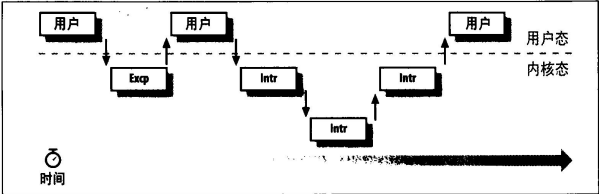
\includegraphics[width=0.6\textwidth]{image/chapter01/内核控制路径.png}
    \caption{内核控制路径的交错执行}
\end{figure}

    上图考虑了以下三种CPU状态:

\begin{itemize}
    \item 在用户态下运行进程(User)
    \item 运行异常处理或系统调用(Excp)
    \item 运行中断处理(Intr)
\end{itemize}

\subsection{进程地址空间}

    \emph{每个进程运行在它的私有地址空间。进程(用户态)涉及到私有栈、数据区和代码区。进程(内核态)涉及数据区和代码区,使用另外的私有栈。}

    因为内核可重入,因此内核控制路径引用自己的私有内核栈。虽然看上去每个进程访问自己的私有地址空间,但是也有共享部分地址空间。

    Linux支持mmap()系统调用,允许存放在块设备上的文件或信息的一部分映射到进程的部分地址空间。

\subsection{同步和临界区}

    实现可重入内核需要利用同步机制:\emph{如果内核控制路径对某个内核数据结构进行操作时被挂起,那么,其他内核控制路径就不应该对该数据结构再操作。除非被设置成一致性\footnote[1]{\emph{一致性状态(Consistency State)是指在分布式系统中,所有副本或节点之间的数据副本保持一致的状态。}}(consistent)状态。否则会破坏所存储的信息。}

    当某个计算结果取决于如何调度两个或多个进程时,相关代码就是不正确的。也就是存在一种竞争条件(race condition)

    一般地,对全局变量的安全访问通过原子操作(atomic operation)来保证。临界区\footnote[2]{\emph{临界区(Critical Section)是指在并发编程中,一段代码或一段程序片段,在同一时间只能被一个线程执行的区域。}}(critical region)就是这样的一段代码,进入这段代码的进程必须完成,之后另一个进程才能进入。

\subsubsection{非抢占式内核}

    在以前,大多数传统Unix内核都是非抢占式的。因此,进程不会被轻易挂起,也不能被随意代替。(单处理器上)中断或异常处理不能修改所有内核数据结构,内核对它们的访问都是安全的。

    内核态的进程需要自愿放弃CPU,但是,必须确保所有的数据结构都处于一致性状态。

    非抢占式在多处理器系统上时低效的,因为运行在不同CPU上的内核控制路径本可以并发访问相同的数据结构。

\subsubsection{禁止中断}

    \emph{(单处理器系统的另一种同步机制)进入临界区之前禁止所有的硬件中断,离开时再启动中断。}尽管机制简单,但是不是最佳的。如果临界区过大,那么在相对长的时间内持续禁止中断会导致硬件活动处于冻结。

\subsubsection{信号量}

    信号量(semaphore)是一种广泛的机制,其仅仅是一个与数据结构相关的计数器。\emph{所有内核线程在试图访问该数据结构之前,需要检查该信号量}。信号量的组成如下:

\begin{itemize}
    \item 一个整数变量
    \item 一个等待进程的链表
    \item 两个原子方法: down()和up()
\end{itemize}

    down()方法对信号量减一,如果新值小于0,则就把正在允许的进程加入信号量链表,然后阻塞该进程(即调用调度程序)。

    up()方法对信号量加一,如果大于等于0,则激活信号量链表中的一个或多个进程。

    每个要保护的数据结构都有自己的信号量,其初始值为1。当内核控制路径希望访问时,调用down(),信号量为非负数允许访问该数据结构。

\subsubsection{自旋锁}

    多处理器中,信号量并不是解决同步的最佳方案。\emph{系统不允许在不同CPU上允许的内核控制路径同时访问某些内核数据结构,这种情况下,修改数据结构所需的事件比较短,而信号量需要加入信号量链表挂起并唤醒,是更为耗时的。}

    因此,多处理器系统使用自旋锁(spin lock)。自旋锁与信号量十分相似,但没有进程链表,当进程发现锁被另一个进程使用时,自身就不停"旋转"。

    注意:\emph{自旋锁在单处理器上是无效的,因为没有机会释放该自旋锁。}

\subsubsection{避免死锁}

    \emph{与其他控制路径同步的进程或内核控制路径很容易进入死锁(deadlock)状态。}

    也就是说:进程p1获得访问数据结构a的权限,进程p2获得访问b的权限,而p1在等待b,p2等待a。

\subsection{信号和进程间通信}

    Unix信号(signal)提供了把系统事件报告给进程的一种机制。每种事件都有自己的信号编号,通常用符号常量表示。有两种系统事件:

\begin{itemize}
    \item 异步通告
    \subitem 例如,用户在中断按下中断键,即向前台发送中断信号SIGINT
    \item 同步错误或异常
    \subitem 例如,进程访问内存地址非法,内核向进程发送SIGSEGV信号
\end{itemize}

    \emph{POSIX标准定义了大约20种不同的信号,其中两种是用户自定义的,可以当作进程通信和同步原语机制。}一般地,进程可以对两种对接方式信号做出反应:

\begin{itemize}
    \item 忽略该信号
    \item 异步地执行一个指定的过程(信号处理程序)
\end{itemize}

    若进程不指定选择何种方式,内核根据编号执行一个默认动作:

\begin{itemize}
    \item 终止进程
    \item 将执行上下文和进程地址空间的内容写入一个文件(核心转储,core dump),并终止进程
    \item 忽略信号
    \item 挂起进程
    \item 如果进程曾被暂停,则恢复执行
\end{itemize}

\subsection{进程管理}

    Unix在进程与执行的程序中做了一个清晰的划分。fork()和\_exit()系统调用分别用来创建和终止进程。exec()类系统调用则是装入新程序。

    执行fork()的进程是父进程,产生的是子进程。\emph{父子进程能够互相找到对方,因为每个描述进程的数据结构都包含两个指针。}

    当前实现fork()的技术是依赖硬件分页单元的内核采用写时复制(Copy-On-Write)技术,即把页的复制延迟到最后(直到父子需要时才写进)。

    \_exit()调用终止进程。通过释放进程所拥有的资源并向父进程发送SIGCHILD信号。

\subsubsection{僵尸进程(zombie process)}

    wait()系统调用允许进程等待,直到一个子进程结束,其返回已终止进程的进程标识符(Process ID, PID)

    引入僵尸进程的特殊状态是为了表示终止的进程:\emph{父进程未执行wait()调用前,其子进程已经终止()。}

    系统调用处理程序从进程描述符字段中获取有关资源的数据,一旦获取,就可以释放进程描述符。

    若父进程终止而没有发出wait()调用,这就会导致该进程一直停留在内存中,无法被使用也无法被清除。因此,可以使用名为init的特殊系统进程(在系统初始化时被创建)。\emph{当一个进程终止时,内核改变其现有子进程的进程描述符指针,将其称为init的子进程,init监视所有子进程的执行,并发布wait(),其作用就是为了除掉所有的僵尸进程}。

\subsubsection{进程组和登录会话}

    现代Unix系统引入了进程组(process group)的概念,以表示一种"作业(job)"的抽象:

\begin{lstlisting}[language=C++]
$ ls | sort | more
\end{lstlisting}

    Shell中为这三个相应的进程创建了一个新的组,就好像它们时一个单独的实体(作业)。每个进程描述符包括一个包含进程组ID的字段。每个进程组可以有一个领头进程(即PID与进程组ID一致)。

    现代Unix系统也引入了登录会话(login session)。非正式的说,一个登录会话包含在指定中断已经开始工作的进程的所有后代进程。

    通常,登录会话时shell为用户创建的第一条命令,进程组中的所有进程必须在同一登录会话中。